\begin{tikzpicture}
\node[inner sep=0,anchor=south west] (im) at (0,0) {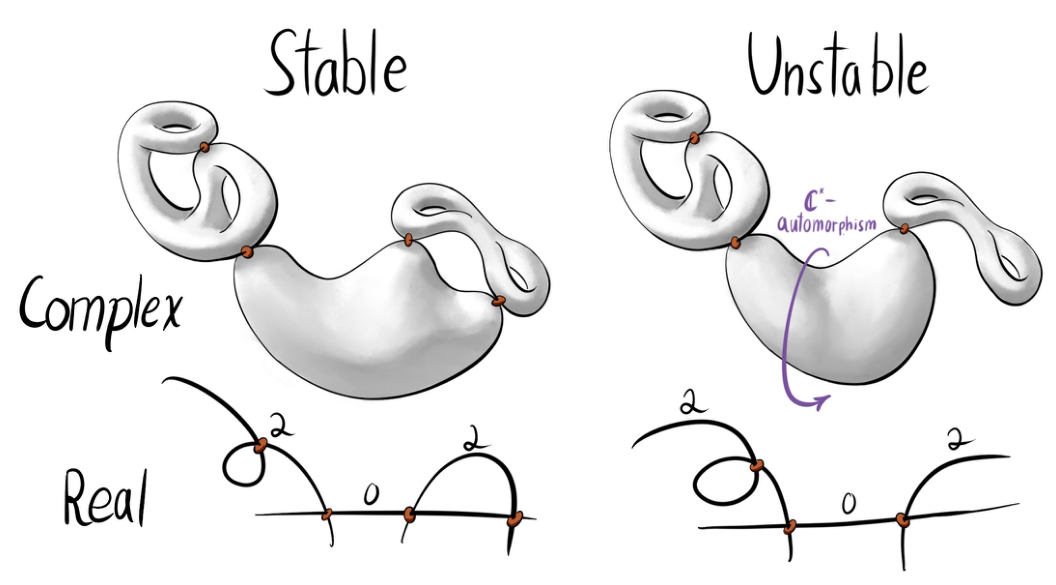
\includegraphics[width=.52\textwidth]{figures/stable-opening.png}};
\begin{scope}[x={(im.south east)},y={(im.north west)}]
\node[fill=white,inner sep=2pt] at (.32,.93) {稳定};
\node[fill=white,inner sep=2pt] at (.76,.93) {不稳定};
\node[fill=white,inner sep=2pt] at (.04,.53) {复};
\node[fill=white,inner sep=2pt] at (.06,.18) {实};
\node[fill=white,inner sep=1pt,font=\tiny,text=violet] at (.77,.69) {$\mathbb C^*$-自同构};
\end{scope}\end{tikzpicture}
